In Abb. \ref{fig: konzept setup} ist ein Sequenzdiagramm dargestellt, das den Ablauf des Konzepts für 
die Einrichtung des erweiterten TOTP-Verfahrens beschreibt. An dem Prozess der Einrichtung nehmen vier Parteien teil. Die App auf dem Smartphone des Nutzers und der Nutzer selbst sowie der Browser als eigene Partei und die Website.

\begin{figure}
    \centering
    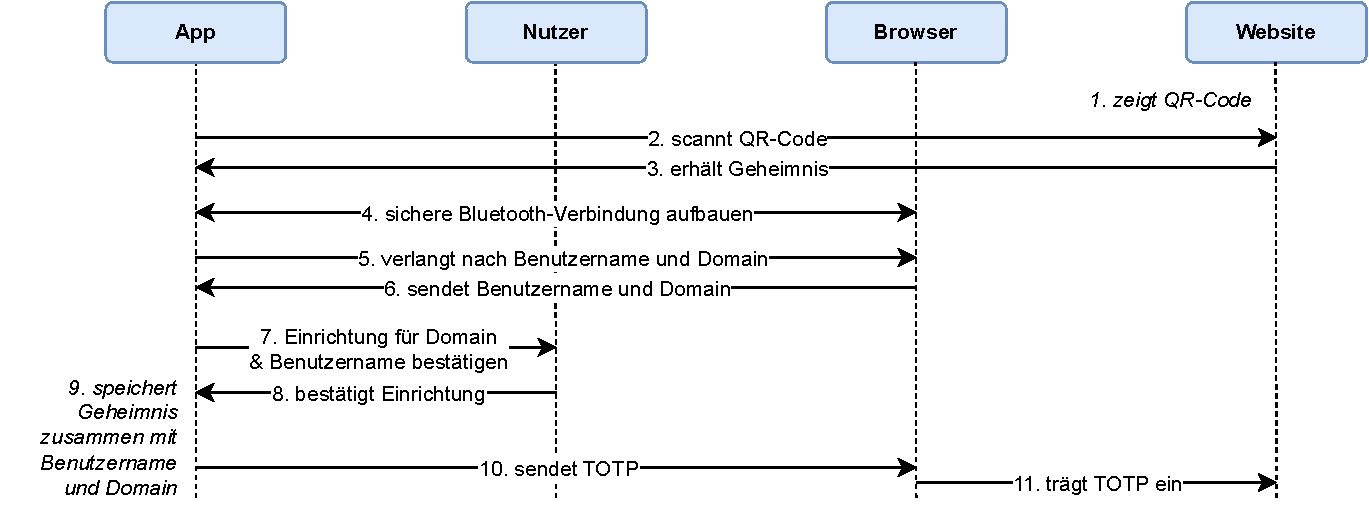
\includegraphics[width=1\linewidth]{figures/konzept_setup.pdf}
    \caption[Einrichtungsprozess des Konzepts zu einem neuen TOTP-Verfahren]{Einrichtungsprozess des Konzepts zu einem neuen TOTP-Verfahren}
    \label{fig: konzept setup}
\end{figure}

\paragraph*{Übertragung des Geheimnisses (1. - 3.)}
\mbox{} \vspace{0.1cm} \\
Üblicherweise wird beim TOTP-Verfahren der QR-Code gescannt, um das Geheimnis von 
der Website in die App zu übertragen. Wenn man das TOTP-Verfahren gänzlich neu 
standardisieren möchte, dann könnte man auch überlegen, ob der Browser den 
QR-Code ausliest bzw. das Geheimnis direkt von der Website erhält, ohne dass der 
Nutzer es sieht. Das Geheimnis könnte dann zusammen mit der Domain des 
Webdienstes und dem Benutzernamen an die App gesendet werden. Möchte man eine 
Lösung implementieren, die den aktuellen Standard nur erweitert, dann bleibt man 
bei der QR-Scan-Methode.

\paragraph*{Aufbau einer sicheren Bluetooth-Verbindung (4.)}
\mbox{} \vspace{0.1cm} \\
Zunächst stellt sich die Frage, welche Art von Bluetooth verwendet werden soll. 
Neben dem Bluetooth Classic bietet sich auch Bluetooth Low Energy (BLE) an, das 
sogar mit dem Web Bluetooth Standard kompatibel ist. Bluetooth bietet 
Sicherheitsfunktionen für eine möglichst sichere Kommunikation an und die 
Bluetooth Special Interest Group (SIG) ist bemüht, die Sicherheit von Bluetooth 
stetig zu verbessern. Allerdings ist eine Ende-zu-Ende-Verschlüsselung auf 
Anwendungsebene empfehlenswert \autocite[9]{siliconLabs} \autocite{androidBt}, da Hardware mit älteren 
Bluetooth-Versionen (bspw. 4.0)  immer noch im Umlauf ist und diese viele 
Schwachstellen aufweisen \autocite{Lonzetta}. Dazu könnte man den Transport Layer Security (TLS) 
Standard nutzen, der jedoch eine Zertifikatskette voraussetzt. Eine andere Lösung 
wäre eine Public-Key-Verschlüsselung, die ggf. beim initialen Schlüsselaustausch 
einige Schwachstellen aufweist, dafür aber unabhängig von Zertifikaten 
funktioniert. Letztendlich sollten die Schutzziele der Informationssicherheit, 
also Vertraulichkeit, Integrität und Verfügbarkeit \autocite[98]{VonSolms}, erfüllt werden. 
Die Bluetooth-Verbindung kann auch schon eher als Schritt 4 
(siehe Abb. \ref{fig: konzept setup}) etabliert werden.
Die Verbindung soll sich 
automatisch wiederherstellen, sobald zwei bekannte Parteien wieder in 
Reichweite sind. Natürlich muss dafür Bluetooth bei beiden Geräte aktiviert sein.

\paragraph*{Benutzername und Domain (5. \& 6.)}
\mbox{} \vspace{0.1cm} \\
Der Browser prüft pro besuchter Domain stetig, ob im HTML-Quellcode ein 
Eingabefeld für den Benutzernamen erscheint. Durch die Popularität von 
Passwort-Managern haben Webdienste auf ihrer Login-Seite meist eine einheitliche 
Markierung gesetzt, damit ein Passwort-Manager programmatisch das Eingabefeld für 
den Benutzername identifizieren kann. Dies funktioniert mit dem HTML-Attribut 
\lstinline{autocomplete}. Es kann verschiedene einheitliche Werte wie \lstinline
{username} für den Benutzernamen annehmen \autocite{htmlAutocomplete}. So kann im 
Konzept der Browser den Benutzernamen feststellen. Sollte es einmal nicht 
funktionieren, dann muss der Browser (oder die App) den Nutzer nach dem 
Benutzernamen fragen.
Die Domain dagegen kann der Browser einfach mit folgendem Javascript-Code 
ermitteln.
\begin{lstlisting}[numbers=none]
let url = document.location.href;
let domain = new URL(url).hostname.replace("www.", "");
\end{lstlisting}

\paragraph*{Bestätigung der Einrichtung (7. \& 8.)}
\mbox{} \vspace{0.1cm} \\
Diese Schritte sind eher optional. So kann der Nutzer noch sichergehen, ob der 
Benutzername korrekt ist und ob er wirklich den Zwei-Faktor-Schutz aktivieren 
möchte. Man könnte dem Nutzer auch erklären, was er bei Verlust des Smartphones 
tun kann.

\paragraph*{Speichern des Geheimnisses (9.)}
\mbox{} \vspace{0.1cm} \\
Die App speichert nun das Geheimnis zusammen mit der Domain und dem Benutzernamen ab. So kann später beim Authentisierungsvorgang mithilfe von Domain und 
Benutzername das notwendige Geheimnis identifiziert werden. Das Geheimnis kann 
verschlüsselt gespeichert werden.

\paragraph*{Übertragung des ersten TOTPs (10. \& 11.)}
\mbox{} \vspace{0.1cm} \\
Traditionell verlangen Dienste nach einem initialen TOTP, um sicherzugehen, dass 
der Nutzer das Geheimnis in seiner App gespeichert hat und der 2FA-Schutz nun 
aktiviert werden kann. Würde man einen neuen Standard entwerfen, könnte man diese 
Schritte auch im Hintergrund erledigen, ohne dass der Nutzer ein Eingabefeld für 
das initiale TOTP sieht. Die App könnte über Bluetooth eine Bestätigung an den 
Browser senden und dieser an die Website.
